\documentclass[12pt]{article}

\usepackage{fullpage}
\usepackage{multicol, multirow}
\usepackage{tabularx}
\usepackage{standalone}
\usepackage{listings}
\usepackage{ulem}
\usepackage{amsmath}
\usepackage{pdfpages}
\usepackage[utf8]{inputenc}
\usepackage[russian]{babel}

\newcommand{\StudentName}{Ильвохин Дмитрий}
\newcommand{\Group}{1O-106М}
\newcommand{\CourseName}{Программирование игр}
\newcommand{\LabNum}{2}
\newcommand{\Subject}{Арканоид}
\newcommand{\PrepName}{Аносова Н.\,П.}

\begin{document}

%\documentclass[a4paper, 12pt]{report}
\usepackage[english, russian]{babel}
\usepackage[utf8]{inputenc}
\usepackage{amssymb, amsfonts, amsmath, mathtext, cite, enumerate, float}
\usepackage{geometry}
\usepackage{chngpage}

\begin{document}

\begin{titlepage}

\newpage

\begin{center}
Московский Авиационный Институт \\*
(национальный исследовательский университет) \\*
Факультет прикладной математики и физики \\*
\hrulefill
\end{center}

\begin{center}
Кафедра вычислительной математики и программирования
\end{center}

\vspace{6em}

\begin{center}
\Large \CourseName \\
	Курсоваой проект \\
  <<\Subject>>
\end{center}

\vspace{2em}
\vspace{6em}

\begin{flushright}
	\StudentName, \\
	группа: \Group \\
\vspace{1em}
преподаватель:\\
   \PrepName \\
\end{flushright}

\vspace{\fill}

\begin{center}
Москва, 2015
\end{center}

\end{titlepage}

\end{document}
 % title page

\lstset
{
        language=Python,
        basicstyle=\footnotesize,% basic font setting
        extendedchars=\true
}

\begin{flushright}
\Large{
	\CourseName \\
	Лабораторная работа №\,\LabNum \\
	<<\Subject>> \\
	%\StudentName, \Group \\
}
\end{flushright}

\subsection*{Задание}
Реализовать игру арканоид.

При столкновеинии ракетки и мяча угол отскока должен меняться в зависимости от места,
куда пришелся удар (удар по центу к изменению не приводит, чем ближе к краю,
тем более пологий угол отскока).

При ударе о ракетку во время достаточно быстрого ее движение угол отражения тоже должен меняться
(вектор движения мяча при отражении складывается с вектором движения ракетки, 
умноженным на некоторый коэффициент) для создания эффекта подкручивания мяча.

\subsection*{Практическая часть}
Как и в первой лабораторной работе Для реализации игры был выбран движок LÖVE (love2d).

В игре игрок контролирует небольшую ракетку, которую можно передвигать горизонтально.
Шарик, отскакивая от ракетки, может разрушить какой-то из еще не разрушенных кирпичиков.
Если все кирпичики разрушены, считается, что игрок победил, если же шарик коснулся пола ---
проиграл.

Самое интересное место в игре --- изменение угла отскока в зависимости от места
столкновения ракетки и шара. За эту часть логики отвечает следующий код:

\begin{lstlisting}
magicDeviationPower = 5
magicReboundPower = 750
function edgeDeviation(ball, racket)
  local ballBody = ball:getBody()
  local racketBody = racket:getBody()
  local racketShape = racket:getShape()
  local dx, dy = ballBody:getLinearVelocity()
  local x_begin, _, x_end, _ = racketBody:getWorldPoints(racketShape:getPoints())
  local racketCenter = (x_begin + x_end) / 2.
  local dir = math.atan2(dy, dx + magicDeviationPower * (ballBody:getX() - racketCenter))
  ballBody:setLinearVelocity
  (
    magicReboundPower * math.cos(dir), magicReboundPower * math.sin(dir)
  )
end
\end{lstlisting}

Дополнительно были реализованы возможности паузы и рестарта игры.

\begin{figure}[!htb]
  \centering
    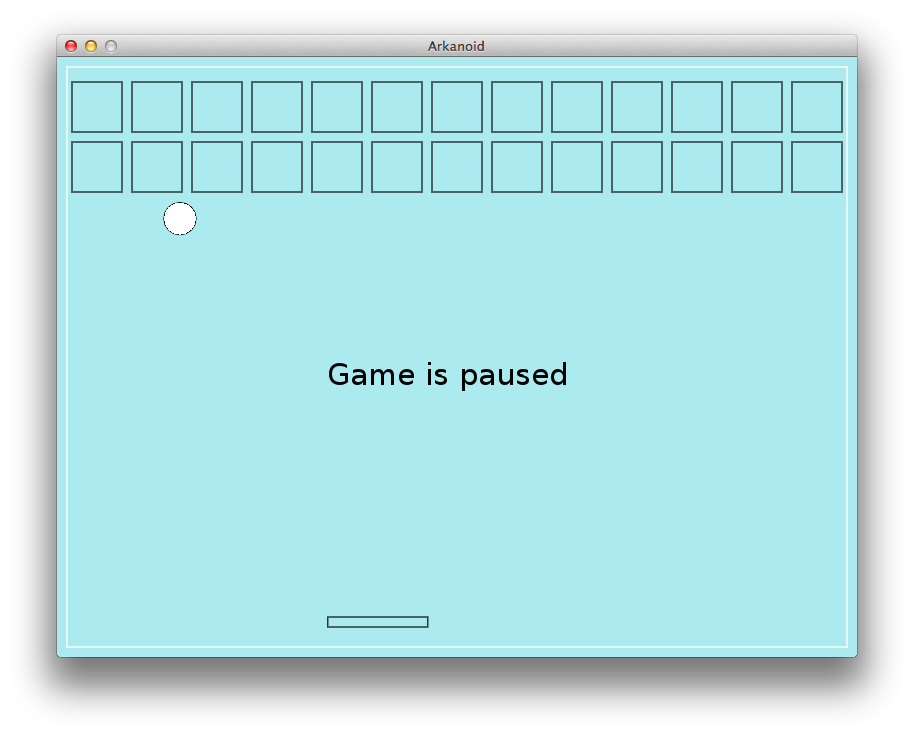
\includegraphics[scale=0.5]{pics/game.png}
   \caption{Скриншот}
    \label{fig:game}
\end{figure}

\subsection*{Выводы}
При выполнении лабораторной чуть лучше познакомился с языком программирования Lua и игровым
движком LÖVE. Кажется, Lua-код этой лабораторной работы выглядит немного лучше, чем код лабораторной работы
№1, что не может не радовать.
\end{document}

